\documentclass[11pt]{article}

\usepackage{setspace}
\usepackage{amsmath}
\usepackage{enumitem}
\usepackage{amsfonts} 
\usepackage{mathtools}
\usepackage{relsize}
\usepackage{graphicx}
\usepackage[top=2cm,bottom=2cm,left=2.5cm,right=2.5cm,marginparwidth=1.75cm]{geometry}
\setlength{\parindent}{0cm}
\usepackage{listings}
\usepackage{clrscode3e}
\usepackage{graphicx}
\def \n {\par \vspace{\baselineskip}}

\def\lc{\left\lceil}   
\def\rc{\right\rceil}
\def\lf{\left\lfloor}   
\def\rf{\right\rfloor}

\title{\vspace{-1.0cm}PHYS 2303 Homework 2}
\author{Fletcher Gornick}
\date{January 28, 2022}

\spacing{1.5}
\begin{document}
 \maketitle 
 \section*{Problem 1-64}
 Rubbing your hands together warms them by converting work into thermal energy. If a
 woman rubs her hands back and forth for a total of 20 rubs, at a distance of 7.50 cm per rub,
 and with an average frictional force of 40.0 N, what is the temperature increase? The mass of
 tissues warmed is only 0.100 kg, mostly in the palms and fingers.
 \newpage

 \section*{Problem 1-79}
 In 1986, an enormous iceberg broke away from the Ross Ice Shelf in Antarctica. It was 
 an approximately rectangular prism 160 km long, 40.0 km wide, and 250 m thick.

 \begin{enumerate}[label=(\alph*)]
   \item What is the mass of this iceberg, given that the density of ice is 917 kg/m\(^3\)?

   \item How much heat transfer (in joules) is needed to melt it?

   \item How many years would it take sunlight alone to melt ice this thick, if the ice absorbs 
     an average of 100 W/m\(^2\), 12.00 h per day?
 \end{enumerate}
 \newpage

 \section*{Problem 1-116}
 A 30.0 g ice cube at its melting point is dropped into an aluminum calorimeter of mass 100.0 g 
 in equilibrium at 24.0 °C with 300.0 g of an unknown liquid. The final temperature is 4.0 °C. 
 What is the heat capacity of the liquid?
 \newpage

 \section*{Probelm 3-28}
 As shown below, calculate the work done by the gas in the quasi-static processes represented by 
 the paths (a) AB; (b) ADB; (c) ACB; and (d) ADCB. \\

 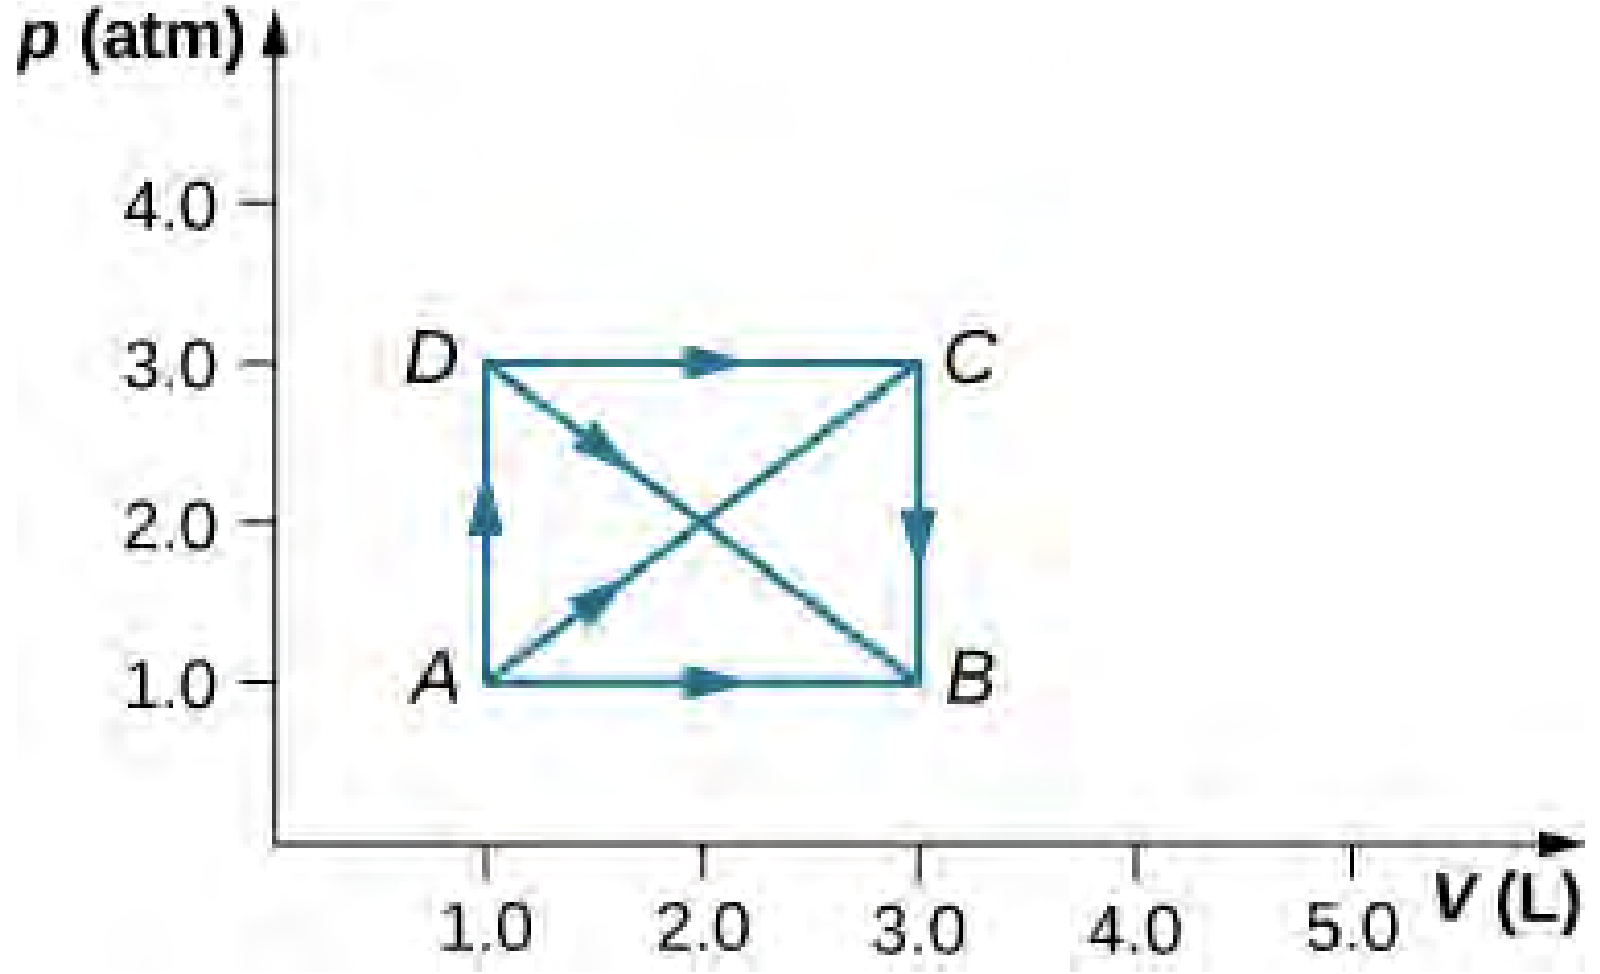
\includegraphics[scale=0.35]{3-28.png}
 \newpage 

 \section*{Problem 3-52}
 A metallic container of fixed volume of \(2.5 \times 10^{-3}\) m\(^3\) immersed in a large tank 
 of temperature 27 °C contains two compartments separated by a freely movable wall. Initially, 
 the wall is kept in place by a stopper so that there are 0.02 mol of the nitrogen gas on one 
 side and 0.03 mol of the oxygen gas on the other side, each occupying half the volume. When the 
 stopper is removed, the wall moves and comes to a final position. The movement of the wall is 
 controlled so that the wall moves in infinitesimal quasi-static steps. 
 \begin{enumerate}[label=(\alph*)]
   \item Find the final volumes of the two sides assuming the ideal gas behavior for the two gases. 
   \item How much work does each gas do on the other? 
   \item What is the change in the internal energy of each gas? 
   \item Find the amount of heat that enters or leaves each gas.
 \end{enumerate}
\end{document}
